\documentclass{article}
\usepackage{amsmath}
\usepackage{tikz}

\begin{document}

\[
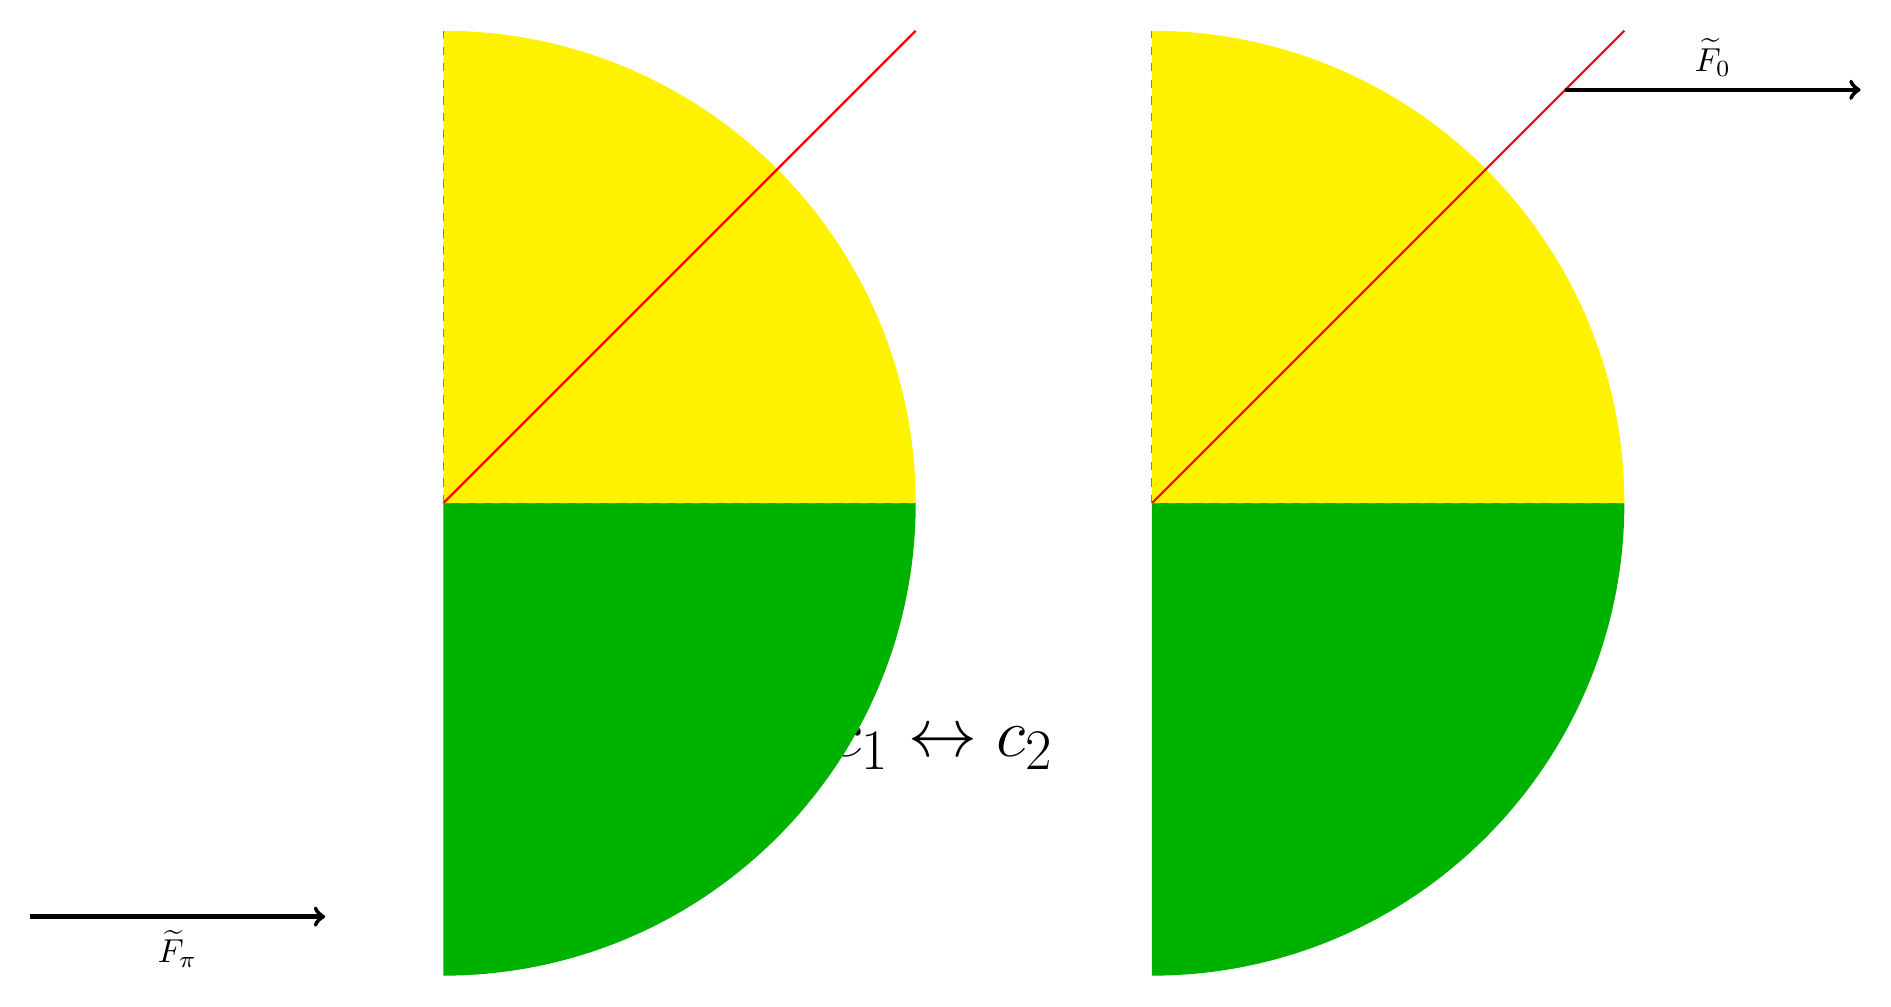
\begin{tikzpicture}[scale=1.5]
    % First half of the diagram
    \fill[yellow] (0,0) -- (0,4) arc (90:0:4) -- cycle;
    \fill[green!70!black] (0,0) -- (4,0) arc (0:-90:4) -- cycle;
    
    \draw[thick,red] (0,0) -- (4,4);
    \draw[dashed,gray] (0,0) -- (0,4);
    \draw[dashed,gray] (0,0) -- (4,0);
    
    % Second half of the diagram
    \draw[->,ultra thick] (3.5,3.5) -- (6,3.5) node[midway,above,scale=1.2] {$\widetilde{F}_{0}$};

    % Third diagram
    \node at (-2,-2) {\Huge$\downarrow c_{1}\leftrightarrow c_{2}$};
    
    \begin{scope}[xshift=-6cm]
        % First half of the third diagram
        \fill[yellow] (0,0) -- (0,4) arc (90:0:4) -- cycle;
        \fill[green!70!black] (0,0) -- (4,0) arc (0:-90:4) -- cycle;
        
        \draw[thick,red] (0,0) -- (4,4);
        \draw[dashed,gray] (0,0) -- (0,4);
        \draw[dashed,gray] (0,0) -- (4,0);
        
        % Second half of the third diagram
        \draw[->,ultra thick] (-3.5,-3.5) -- (-1,-3.5) node[midway,below,scale=1.2] {$\widetilde{F}_{\pi}$};
    \end{scope}
\end{tikzpicture}
\]

\end{document}